\subsection{Age structure and public transfers}

Public transfers are inter-generational; this involves collecting resources from the working-age population (the outflow transfers) and reallocating them to the dependent population, mostly the young and old (the inflows transfers).
The immigrant and native populations are different not only in their size but also in their age structure.
By dividing total (across all ages) transfer by the total population, per-capita comparison between immigrant and natives accounts for the difference in the population size but not for the difference in age structure.
It follows that a comparison based on per-capita values is biased to the extent that the two populations have different age structures.
To account for this biais, the decomposition discussed earlier is applied to the surpluses in each account and sub-account separately .
The decomposition function takes the age-specific transfer and the population size as inputs for a given transfer account. It then applies the decomposition algorithm and returns the two components representing the respective contributions of the inputs to the per capita crude surplus.
Doing so allows extracting the share of crude surplus accrued by a difference in age-specific transfer rather than a difference in the age structure of the two populations.

\vspace{0.7em}\par
Age-adjusted surpluses are the components associated with age-specific transfers and represent the difference between an immigrant and a native of the same age.
We will also refer to these as fiscal components
On the other hand, demographic components are associated with the population size by age.
However, they express only the portion of the surplus that results from a difference in the age structure between the two populations because the per-capita calculation cancels out the effect of the total population size.
Also, as Net Surplus is the sum of all Immigrant Surpluses across all accounts (inflows minus outflow), the age-adjusted Net Surplus is computed similarly, as the sum of all age-adjusted Immigrant Surpluses. \autoref{fig:DEcomp} presents the trend in the crude and age-adjusted surpluses as well as the demographic components for each sub-accounts throughout the studied period.
Account names are simplified as per \autoref{tab:tx2015}

\begin{figure}[H]%
  \caption{Trend in Immigrant Surpluses for crude transfer (perCapita) and its age-adjusted (Adj.Transfer) and demographic components(Age.Structure) by transfer accounts, Canada 1997-2015.}
  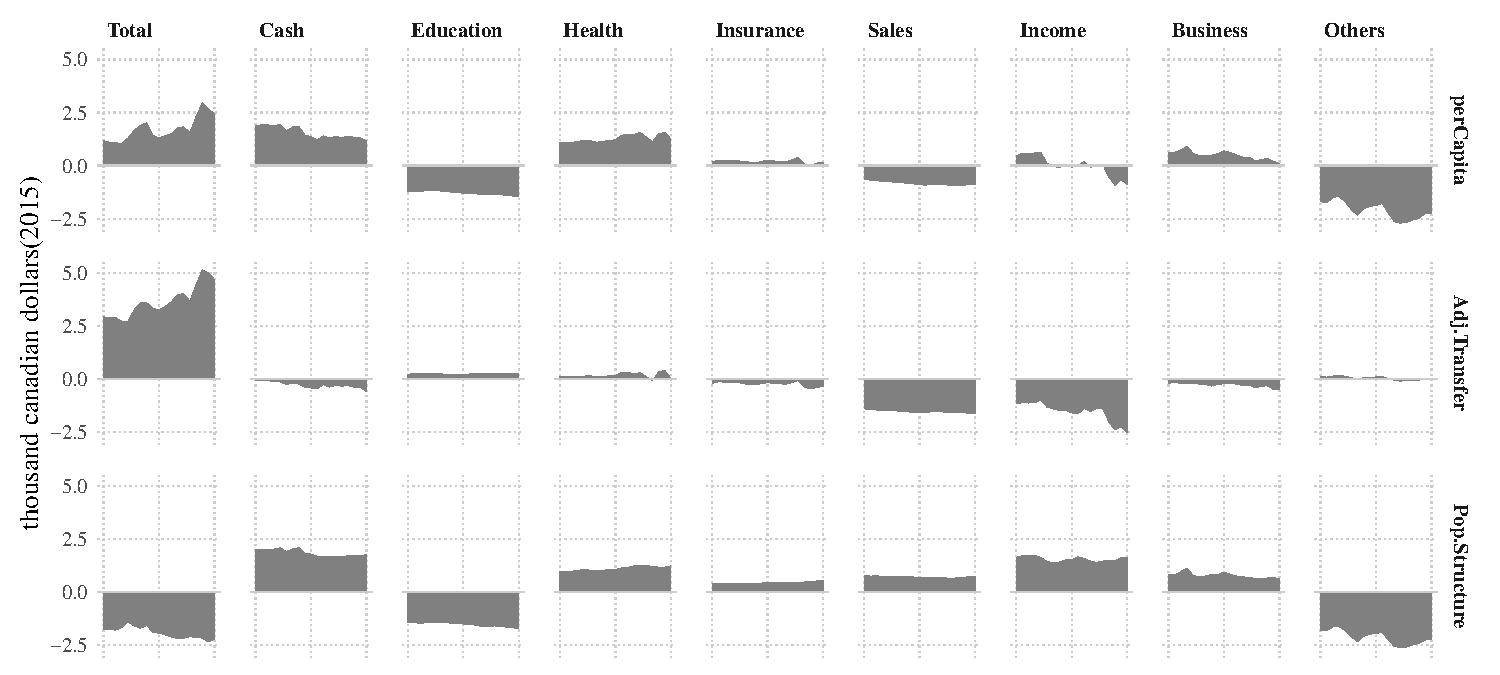
\includegraphics[width=1\textwidth]{../ntaImmig/res/DEcomp.pdf}%
  \label{fig:DEcomp}%
\end{figure}%

\subsection{Age-adjusted Net Surplus}

Results show that age-adjusted Net Surplus followed the same pattern as per-capita Net Surplus, but the levels are much higher in absolute values.
Furthermore, the overall negative sign for demographic components of Net Surplus indicates that age structure is much more favourable to immigrants, as it reduced the difference between immigrants and natives from the adjusted value to the per-capita value.
In other words, the per-capita difference would have been much higher than its current (crude) value if the immigrant and native populations had the same age structure.
In dollar value, at equal age, the average immigrant has cost to the state about \$\numUp{AveAdj.Transfer} per year, more than the average native, between 1997 and 2016.
However, a favourable population structure reduced this surplus by about \$\numUp{AvePop.Structure}, leading the \$\numUp{AveperCapita} in per-capita Net Surplus.
While the demographic effect has increased steadily during the studied period from \$\numUp{AvePop.Structure1997} to \$\numUp{AvePop.Structure2015}, the trends in Adjusted Net Surplus were much abrupt with increases every few years (early 2000, late 2000, early 2010) from \$\numUp{AveAdj.Transfer1997} in 1997 to \$\numUp{AveAdj.Transfer2015} in 2015.
The steady increase of the demographic components over the years reflects the faster ageing of the native population, as the immigrant population has been purposefully kept young through various economic immigration programs.

\vspace{0.7em}\par
These results imply that the difference in age structure between immigrant and native populations accounts for much of their difference in crude surpluses.
Therefore, not accounting for the demographic effect leads to conflicting results that confuse our understanding of the transfer differential between immigrants and natives, create unnecessary discord in the immigration debates, and lead to inappropriate public policy.
The confusion goes even further when comparing the sub-account of inflow and outflow as we shall see in the following section.

\subsection{Age-adjusted surpluses in sub-accounts}

Looking at the adjusted surplus for the sub-accounts, it appears that income and sales taxes are the primary sources of the Net Surplus.
This result makes sense because the other sub-accounts tied to public programs are less likely to increase social inequality to the size of the Immigrant Surplus.
On the other hand, the sub-accounts of Income and Sales taxes directly relate to individual revenue, which is more subjected to labour market outcomes than public policy.
However, this pattern is not observable from the crude values, and crude Net Surplus shows opposite results, with inflows appearing as the primary sources of disparities in Net Transfers.
For example, most contributions to public finances represent a given proportion of the individual's income.
Therefore, it is intuitive that the sub-account of income taxes reflects the difference between immigrants and natives to a large extent.
On the contrary, the crude Net Surplus for income taxes shows conflicting results, positive between 1997 and 2003, null till 2012, and negative afterward.

\vspace{0.7em}\par
These results illustrate the mitigating effect of demographic components in the differences in transfer between immigrants and natives.
Demographic differences are also the reasons for the high per-capita health care cost, which is close to zero in the age-adjusted surplus.
In other words, the high difference in health care transfer between immigrants and natives implies that there are relatively more immigrants in the age groups with the highest health care costs.
This implication may be unexpected since the average age of new immigrants entering Canada is lower than the average of the native population.
But as shown by \citet[p~244]{Malenfant.2011}, the immigrant population in Canada is older than the population as a whole because immigrants are over-represented above the age of 30 and under-represented below.

\vspace{0.7em}\par
Not only have demographic differences affected the size of the Immigrant Surplus, but they have also changed its direction and trend.
For example, looking at the per-capita surplus, immigrants seem to have paid on average more business taxes than natives.
However, after adjusting for demographic effects, the situation reverses, with immigrants paying fewer business taxes than natives. Moreover, contrary to the per-capita measure, the trend in Immigrant Surplus is increasing.
The low business taxes paid by immigrants suggest that they operate smaller businesses than natives.
They also contributed toward social security and received cash transfers, slightly less than natives.
The opposite applies to education and health care costs, where immigrants consume slightly more than natives.

\vspace{0.7em}\par
The Other sub-account of transfer includes public goods, services, deficits and debts.
The NTA method distributes these costs evenly, making no difference between immigrants and natives by design.
As a result, the age-adjusted surplus for the other sub-accounts is close to zero and has the lowest absolute value among all sub-accounts.
Therefore the significant negative effect (in favour of natives) seen in the per-capita surplus is mainly due to the difference in age structure between immigrants and natives.
When adjusted for these differences, the surpluses in these other sub-accounts compensated each other, revealing the sub-account of sales and income taxes as the two most important sources of disparities between immigrants and natives.

\vspace{0.7em}\par
Immigrants receive similar benefits from public programs, but their low revenue does not contribute equally to public finances, leading to a positive Net Surplus.
As a result, difference in sales and income taxes added up to an age-adjusted surplus of \$\numUp{SIAdjusted} which represent \numUp{SIprop}\% of the \$\numUp{AveAdj.Transfer} in total age-adjusted surplus.
As these taxes come from income mainly earned from labour, the labour market stands out as a significant source of inequality between immigrants and natives.
Furthermore, while both income and sales taxes are the main contributors to Net Surplus, income taxes alone drive its trends.
These results stand against the expectations of a positive impact of immigration on public finances, especially for recent immigrants for whom economic factors have motivated admission.
However, there are not revealed until demographic differences between immigrants and natives are accounted for.
Therefore, how the labour market has become the source of so many imbalances, especially since 2011, is a crucial question to discuss and address should Canada intend to benefit from its immigrants.
In particular, understanding how hiring and wage discrimination affect immigrants' contribution to society and government revenues will be essential.

















